\section{Additional Stress Results}
\label{app:norm_ablation}
\begin{table}[t]
\centering
\caption{Synthetic scale stress (02): Macro Score across scale factors. Mean $\pm$ std over 10 seeds.}
\label{tab:stress_scale}
\resizebox{\columnwidth}{!}{%
\begin{tabular}{l c c c c}
\toprule
Method & $\times{1}$ & $\times{10}$ & $\times{100}$ & $\times{1000}$ \\
\midrule
Kendall & $0.738 \pm 0.017$ & $\mathbf{0.607 \pm 0.038}$ & $0.522 \pm 0.030$ & $0.499 \pm 0.025$ \\
UWSO & $0.690 \pm 0.034$ & $0.604 \pm 0.040$ & $0.525 \pm 0.035$ & $0.494 \pm 0.024$ \\
BPGS & $\mathbf{0.743 \pm 0.018}$ & $0.616 \pm 0.039$ & $\mathbf{0.547 \pm 0.032}$ & $\mathbf{0.543 \pm 0.032}$ \\
\bottomrule
\end{tabular}
}
\end{table}

\begin{table}[t]
\centering
\caption{Relative Macro Score change (\%) from $\times 1 \to \times 1000$. Positive values indicate degradation; negative values indicate improvement.}
\label{tab:degradation}
\begin{tabular}{l c c}
\toprule
Method & Scale Stress & Loss Rescaling \\
\midrule
Kendall & $32.3\%$ & $18.4\%$ \\
UWSO & $28.5\%$ & $\mathbf{-9.5\%}$ \\
BPGS & $\mathbf{27.0\%}$ & $0.0\%$ \\
\bottomrule
\end{tabular}
\end{table}

\begin{table}[t]
\centering
\caption{Heterogeneous mixed stress: Macro Score and Worst-Task Score across regimes. Mean $\pm$ std over 3 seeds.}
\label{tab:stress_heterogeneous}
\resizebox{\columnwidth}{!}{%
\begin{tabular}{l c c c c c c}
\toprule
Method & \multicolumn{2}{c}{Clean} & \multicolumn{2}{c}{Noisy} & \multicolumn{2}{c}{Conflict} \\
& Macro & Worst & Macro & Worst & Macro & Worst \\
\midrule
Kendall & $0.687 \pm 0.010$ & $0.267 \pm 0.056$ & $\mathbf{0.659 \pm 0.007}$ & $\mathbf{0.242 \pm 0.045}$ & $\mathbf{0.664 \pm 0.012}$ & $\mathbf{0.211 \pm 0.041}$ \\
UWSO & $0.437 \pm 0.028$ & $0.000 \pm 0.000$ & $0.438 \pm 0.020$ & $0.000 \pm 0.000$ & $0.433 \pm 0.013$ & $0.000 \pm 0.000$ \\
PCGrad & $\mathbf{0.688 \pm 0.016}$ & $0.274 \pm 0.055$ & $0.656 \pm 0.007$ & $0.241 \pm 0.046$ & $0.660 \pm 0.011$ & $0.205 \pm 0.048$ \\
BPGS & $0.679 \pm 0.017$ & $\mathbf{0.301 \pm 0.052}$ & $0.641 \pm 0.013$ & $0.176 \pm 0.076$ & $0.652 \pm 0.012$ & $0.198 \pm 0.063$ \\
\bottomrule
\end{tabular}
}
\end{table}
\begin{table}[t]
\centering
\caption{Normalization ablation on pure loss rescaling. Macro score (mean $\pm$ std over seeds 42, 123, and 999). L1-normalizing Kendall improves the largest-scale result but does not reproduce the BPGS scale sensitivity.}
\label{tab:norm_ablation}
\small
\begin{tabular}{lccc}
\toprule
Scale & BPGS & Kendall & Kendall+L1 \\
\midrule
$\times1$    & $0.789 \pm 0.018$ & $0.788 \pm 0.014$ & $0.794 \pm 0.017$ \\
$\times10$   & $0.791 \pm 0.015$ & $0.781 \pm 0.023$ & $0.780 \pm 0.022$ \\
$\times100$  & $0.788 \pm 0.016$ & $0.734 \pm 0.037$ & $0.742 \pm 0.029$ \\
$\times1000$ & $0.785 \pm 0.017$ & $0.658 \pm 0.042$ & $0.689 \pm 0.034$ \\
\midrule
$\Delta(\times1\!\to\!\times1000)$ & $-0.004$ & $-0.130$ & $-0.105$ \\
\bottomrule
\end{tabular}
\end{table}


\begin{figure*}[t]
\centering
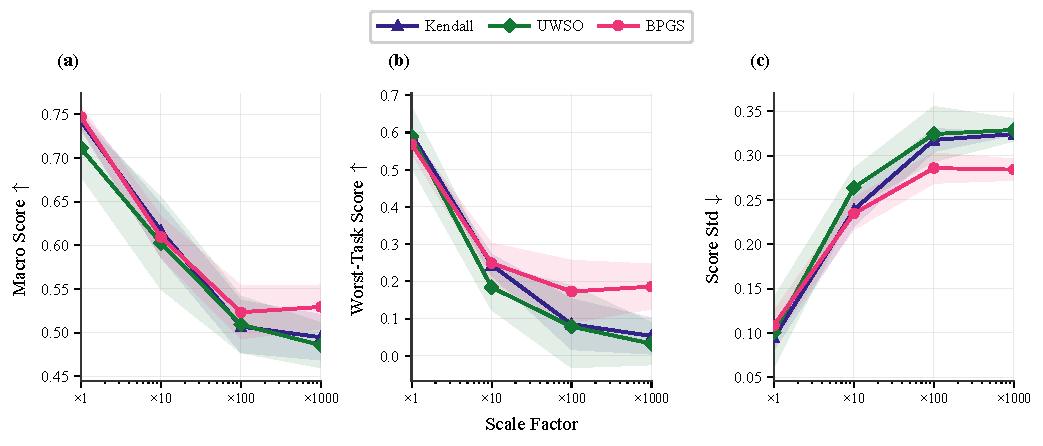
\includegraphics[width=\textwidth]{data/stress/scale/figures/pdf/scale_stress_curves.pdf}
\caption{Synthetic scale-stress curves. As the scale factor increases, all methods degrade, but BPGS retains the strongest macro score at every tested factor and tracks the strongest worst-task score at the larger stress levels.}
\label{fig:appendix_scale_stress}
\end{figure*}

\begin{figure*}[t]
\centering
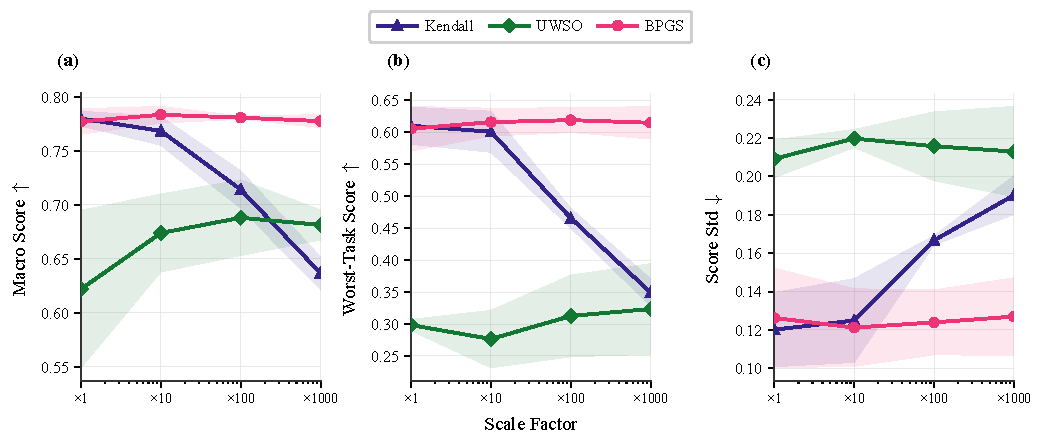
\includegraphics[width=\textwidth]{data/stress/rescaling/figures/pdf/rescaling_stress_curves.pdf}
\caption{Pure loss-rescaling curves. BPGS remains nearly invariant across the entire rescaling range, while Kendall degrades sharply at larger factors and UWSO improves only from a substantially weaker starting point.}
\label{fig:appendix_rescaling}
\end{figure*}

\begin{figure*}[t]
\centering
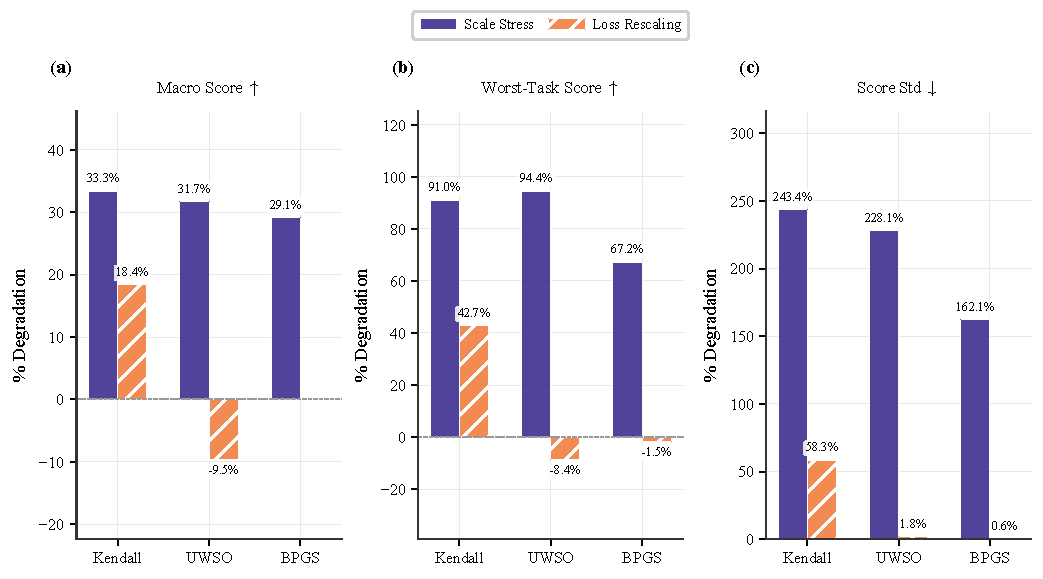
\includegraphics[width=\textwidth]{data/stress/combined/figures/pdf/degradation_comparison.pdf}
\caption{Relative degradation comparison between synthetic scale stress and pure loss rescaling. The figure shows that BPGS has the smallest macro-score degradation under scale stress and essentially no macro-score degradation under pure rescaling.}
\label{fig:appendix_degradation}
\end{figure*}

\begin{figure*}[t]
\centering
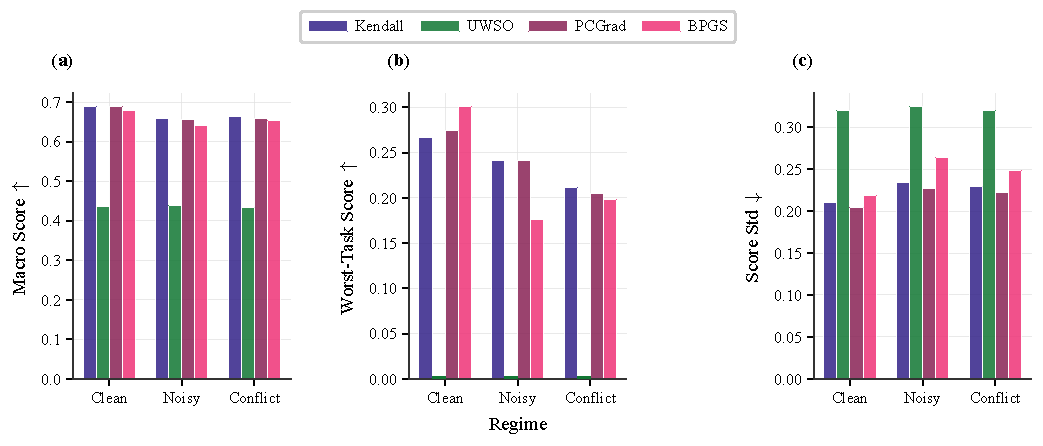
\includegraphics[width=\textwidth]{data/stress/heterogeneous/figures/pdf/heterogeneous_panel.pdf}
\caption{Heterogeneous mixed-stress summary. BPGS is not the best method in every regime, but it achieves the strongest worst-task score in the clean regime and remains well above the degenerate UWSO worst-task score across all regimes.}
\label{fig:appendix_heterogeneous}
\end{figure*}
